\section{The Gr\"obner Fan of an ideal: A mix of commutative algebra,
  combinatorics, and linear programming}

For this discussion, we will choose to represent monomial orders as matrices with
real entries. There are different conditions for particular entries in such matrices
to define a monomial order \cite{Cox:2014}.

In order to compare two terms it is just necessary to use their exponents. Let $M$
be a matrix and $\alpha, \beta$ the exponents of two polynomials.
A matrix order works as follows: $\alpha \prec_M \beta$
if there exists a row vector $\omega$ in $M$, say the ith row, such that
$\alpha \cdot \omega < \beta \cdot \omega$ and all previous rows $\omega^{'}$ in $M$
we have that $\alpha \cdot \omega^{'} = \beta \cdot \omega^{'}$.

\begin{example} Let us consider the following matrix
  $M = \begin{pmatrix} 1 & 1 & 1 \\
    1 & 0 & 0 \\
    0 & 1 & 0 \\
    0 & 0 & 1 \end{pmatrix}$. This matrix encodes the \emph{graded lexicographical
    order} $x > y > z$ for the polynomial ring $k[x, y, z]$. We can see that the first row
  essentially compares the total grade in the exponent of terms and the rest
  of the rows break tie using the lexicographic order.
\end{example}

\begin{example}
  On the other hand, not all matrices define a monomial order. For instance, let
  us consider the matrix $M^{'} = \begin{pmatrix} 1 & 2 & -1 & -2 \\
    2 & -1 & -2 & 1 \\
    -1 & -2 & 1 & 2 \\
    -2 & 1 & 2 & -1
  \end{pmatrix}$. We notice that multiplying $M^{'}$ with any vector with the same elements in each
  entry will give us a zero vector. Hence $M^{'}$ cannot distinguish
  these set of vectors, which is problematic according to the definition
  of a monomial order. In general it should be desirable that the kernel
  of these matrices intersecting the correspondant $\nat^n$ is empty.
  The latter will provide injectivity to the matrix in order to distinguish
  different vectors. The latter property is common and shared among different
  monimonial order in different domains (rational, real) of matrices.
\end{example}

We will like to study Gr\"obner bases without \emph{explicitly}
specifying the monomial ordering. For the latter the idea of a
\emph{marked Gr\"obner basis} was introduced.

\begin{definition} \cite{Cox:2014}
  A \emph{(reduced) marked \grob basis} is a set of pairs of polynomials and monomials
  $\{(f_i, g_i) | i = 1, \dots, r\}$ such that $\{f_i | i = 1, \dots, r\}$ is
  a (reduced) \grob basis and $g_i = LT_\prec(f_i)$ for some monomial order $\prec$.
\end{definition}

The latter definition helps providing an implicit monomial ordering,
i.e. the monomial order used to compute the \grob basis is not available.
Is this information enough to uniquely determine the original
monomial order used to compute the \grob basis? As shown in \cite{Cox:2014},
having the information of the leading monomial we can produce a set of
inequalities that, if satisfiable, the solution of such system of inequalities
corresponds to the first row of matrix order.

\begin{example} We will highlight the leading monomial of a polynomial using parenthesis.
  Let us consider the marked \grob basis $\{(xy)-z^2, (wyz)-x^3, (wy^2)-x^2z, (wz^3)-x^4\}$.
  The set of inequalities entailed by the marked \grob basis is:
  \begin{itemize}
  \item $(0, 1, 1, 0) \cdot (a, b, c, d) \geq (0, 0, 0, 2) \cdot (a, b, c, d)$
  \item $(1, 1, 1, 0) \cdot (a, b, c, d) \geq (0, 3, 0, 0) \cdot (a, b, c, d)$
  \item $(1, 0, 2, 0) \cdot (a, b, c, d) \geq (0, 2, 0, 1) \cdot (a, b, c, d)$
  \item $(1, 0, 0, 3) \cdot (a, b, c, d) \geq (0, 4, 0, 0) \cdot (a, b, c, d)$
  \end{itemize}
  Using a linear solver we compute a solution for the above system of inequalities:

  \begin{figure}[h]
    \centering
    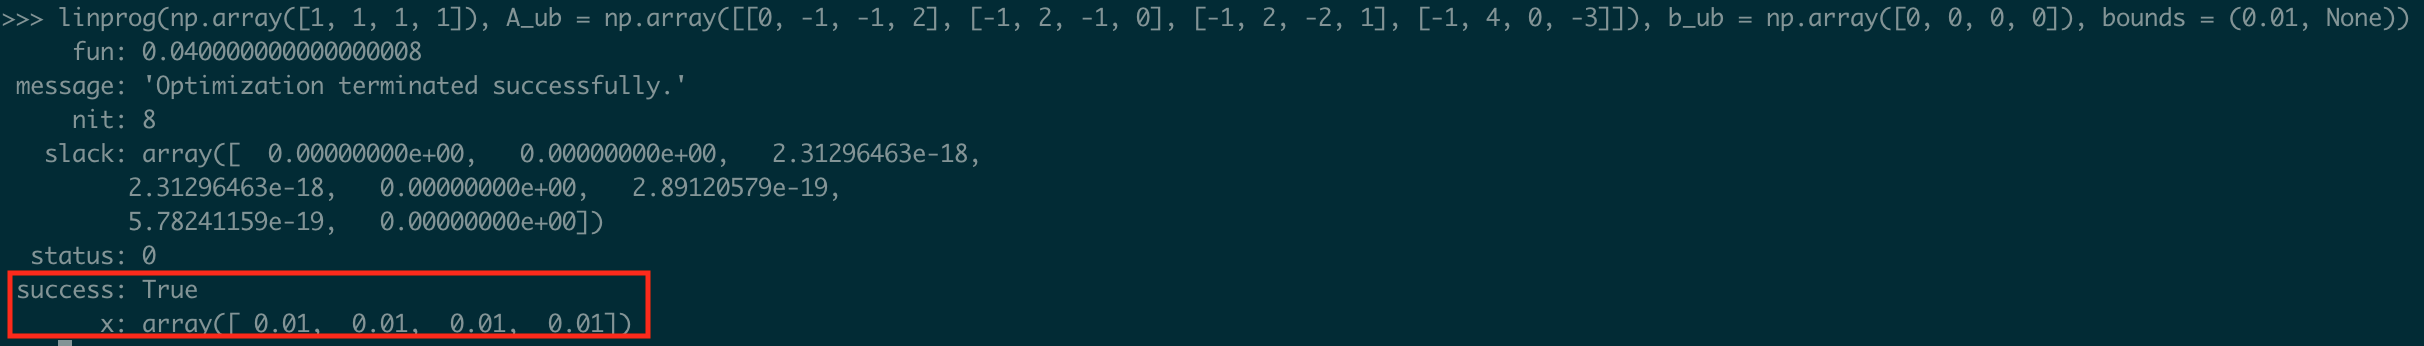
\includegraphics[width=15cm]{example1}
    \caption{The solution found by scipy.optimize.linprog \cite{linprog} is $x = [0.01, 0.01, 0.01, 0.01]$}
  \end{figure}
\end{example}

We notice then that the first row for the previous matrix order are all the same elements. Thus we can suspect
an equi-graded order (i.e. an order which doesn't prefer an indeterminate while computing the total
grade) is used. This phenomenon happens quite frequently, specifically with equi-graded orders. For example,
consider the graded lexicographical order $x > y > z$ and the graded lexicographical order $y > z > x$. The first
row of their matrix order will be the same, but the rest of their matrices will be different.

From the previous observation, if we take all the vectors in the $\real^n$ such that they satisfy the set of
inequalities demanded by a matrix order we will obtain a \emph{cone} in $\real^n$. In \cite{Cox:2014} it is
shown that the geometry properties of these cones form a fan, which is a structure such that the intersection
of cones (known as faces) belong to the structure as well as each of the faces of the cones belong to the
structures. In hindsight, the faces of this structure correspond to elements of the cones such that the
the dot product cannot distinguish between exponent vectors, hence it is important to rely on the interior
points of these cones to fully distinguish/classify exponent vectors. 

%%% Local Variables:
%%% mode: latex
%%% TeX-master: "main"
%%% End:
